\chapter{Method}\label{ch:method}
\Todo{maybe name this chapter smth else??}

A combination of the methods described in Chapter \ref{ch:theory} is proposed in the present study.


\section{Chuck language}
\textbf{Chuck} language is a music programming language, made for ``real-time sound synthesis and music creation'' as mentioned in their website \cite{bib:chuck}. It's biggest advantage is the way it manipulates time. More specifically, the user specifies how long a sound will last, independent of other sounds that may play at the same time.

\paragraph{Modal features extraction code\\}
We used the ChucK language at the starting point of our thesis to identify and extract the peaks of the recorded ``wav'' files. The algorithm used in this part of the thesis is made by Perry Cook for the course \textbf{``Physics-Based Sound Synthesis for Games and Interactive Systems''} held by \textit{Perry Cook} and \textit{Julius O. Smith} at \textbf{Kadenze Academy} \cite{bib:physicsbasedcourse}.

From a FEM analysis one can find out that each object vibrates in a very high number of modes. Although, most of them are inaudible and do not contribute to the sound model. Thus, we can easily define \textit{ten} to be the total number of peaks identified. After some trials, we found out that \textit{five} peaks are already enough. However, the authors recommend to use twice the sufficient number, hence \textit{ten} for our case. Afterwards, the algorithm having taken a recording as input, computes its histogram and identifies its peaks. The frequencies where peaks occur are the modal frequencies candidates. Depending on the numbers of peaks we chose, the algorithm outputs a normalization between high and low peaks. Finally, the algorithm finds the maximum value of the signal on each peak, calculating the corresponding amplitude of each mode.

 
\section{PureData}
\textbf{Pure Data (pd)} is another music programming language. It is open source and the main difference from ChucK language is that pd is a visual or ``patcher'' programming language, using objects instead of code, linked together to form a sequence \cite{bib:pd}.

\paragraph{Re-synthesis patch\\}
For reasons that will be explained below, we had to attach only one pd patch to every 3D object in the demo. Therefore, all synthesized sounds (impact, rolling and scratching) are being synthesized under one main pd patch. 

The main part of the re-synthesis patch is the resonator. Using band-pass filters it gives the impulse response of an object struck at a specified point. It also clips the signal to give more brightness and harmonics. \Todo{develop more}

\section{Heavy Compiler}
\textbf{Heavy} is a compiler that generates audio plugins from pd patches in interactive soudn and music applications \cite{bib:heavy}. In this thesis we used it to compile pd patches into Unity audio plugins. Heavy's interface is their website where users upload patches and then are able to download the corresponding plugins and put them into their applications. The plugins we used consist of DLL files and a C\# (Unity code) script that allows communication of the plugins with the rest of the script and also enables the sound card to play sounds.

\section{Unity\textregistered}
\textbf{Unity\textregistered} is a game engine software. This is where all previous work is combined together and gives the final product. For the purpose of this thesis, a sample scene is made inside unity where objects are struck in several points and produce different sounds. 

The first part of the Unity implementation is the assignment of modal data to every different area of the object. This is done in $O(n)$ time for $n$ modes. Since we only used simple shape everyday objects, we could easily assume that nearby points produce almost the same sound and thus separate the object into ``modal areas'' instead of calculating different modal matrices for each point. Tests in users proved that this accuracy-computational complexity trade-off was acceptable.  

\section{Microsoft Hololens Emulator}

\section{Overview of our tool}
\Todo{replace figure  with a better one}
\begin{figure}[H]
  \centering
    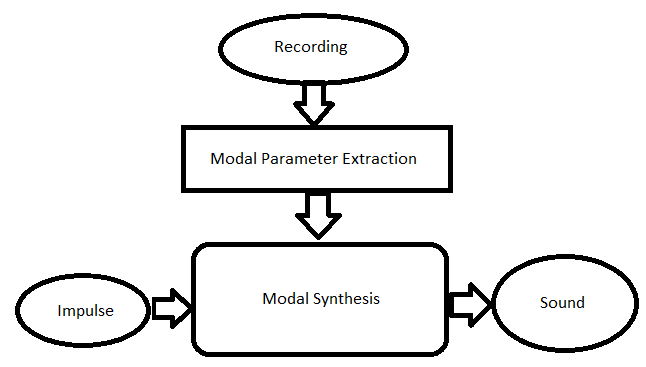
\includegraphics[width=0.5\textwidth]{synthesisChart.png}
      \caption{Sound Synthesis Procedure.}
      \label{fig:synth_proc}
\end{figure}